\tableofcontents\clearpage

\section{Wstęp}
\subsection{Cel ćwiczenia}
\hspace*{0.5cm}Celem ćwiczenia było stworzenie układu realizującego funkcje licznika, wyświetlającego cyfry na wyświetlaczu siedmio segmentowym. Układ ma posiadać funkcję dwóch przycisków: Reset i Stop, a ich sposób implementacji jest dowolny. \\ \hspace*{0.5cm}Układ również powinien być zaprojektowany segmentowo, czyli każda funkcjonalność powinna być osobnym elementem. Napisane oczywiście w języku VHDL.

\vspace*{0.5cm}

\hspace*{0.5cm}W późniejszych pod-działach poszczególnych elementów ,,Działanie'' zostanie krótko opisana ich funkcjonalność. 

\subsection{Graficzne przedstawienie schematu}
\begin{figure}[!htb]
    \centering
    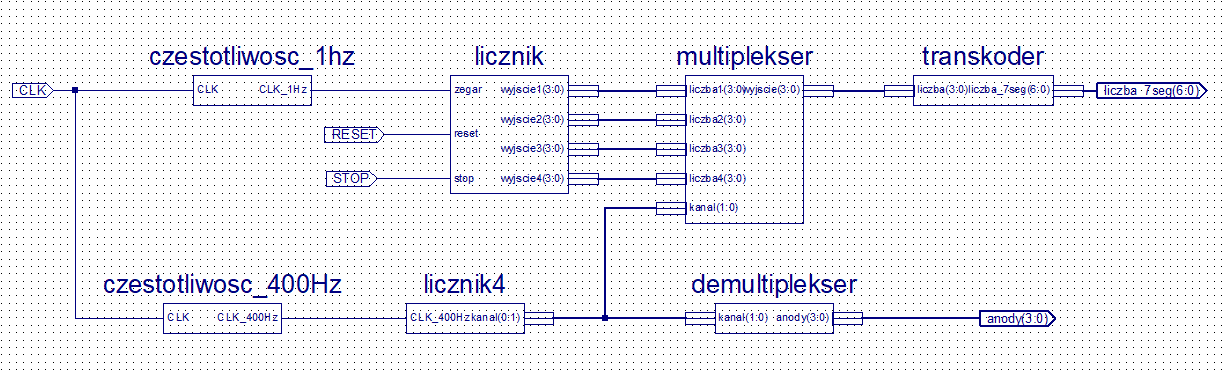
\includegraphics[width=18.4cm]{./Kod/schemat.png}
    \caption*{schemat układu VHDL}
\end{figure}

\subsection{Połączenie elementów przy pomocy kodu}
\begin{lstlisting}
    library ieee;
    use ieee.std_logic_1164.ALL;
    use ieee.numeric_std.ALL;
    library UNISIM;
    use UNISIM.Vcomponents.ALL;
    
    entity schemat is
       port ( CLK         : in    std_logic; 
              RESET       : in    std_logic; 
              STOP        : in    std_logic; 
              anody       : out   std_logic_vector (3 downto 0); 
              liczba_7seg : out   std_logic_vector (6 downto 0));
    end schemat;
    
    architecture BEHAVIORAL of schemat is
       signal XLXN_1      : std_logic;
       signal XLXN_2      : std_logic;
       signal XLXN_3      : std_logic_vector (3 downto 0);
       signal XLXN_4      : std_logic_vector (3 downto 0);
       signal XLXN_6      : std_logic_vector (3 downto 0);
       signal XLXN_7      : std_logic_vector (3 downto 0);
       signal XLXN_9      : std_logic_vector (1 downto 0);
       signal XLXN_10     : std_logic_vector (3 downto 0);
       component licznik
          port ( zegar    : in    std_logic; 
                 reset    : in    std_logic; 
                 stop     : in    std_logic; 
                 wyjscie1 : out   std_logic_vector (3 downto 0); 
                 wyjscie2 : out   std_logic_vector (3 downto 0); 
                 wyjscie3 : out   std_logic_vector (3 downto 0); 
                 wyjscie4 : out   std_logic_vector (3 downto 0));
       end component;
       
       component multiplekser
          port ( liczba1 : in    std_logic_vector (3 downto 0); 
                 liczba2 : in    std_logic_vector (3 downto 0); 
                 liczba3 : in    std_logic_vector (3 downto 0); 
                 liczba4 : in    std_logic_vector (3 downto 0); 
                 kanal   : in    std_logic_vector (1 downto 0); 
                 wyjscie : out   std_logic_vector (3 downto 0));
       end component;
       
       component demultiplekser
          port ( kanal : in    std_logic_vector (1 downto 0); 
                 anody : out   std_logic_vector (3 downto 0));
       end component;
       
       component licznik4
          port ( CLK_400Hz : in    std_logic; 
                 kanal     : out   std_logic_vector (0 to 1));
       end component;
       
       component czestotliwosc_1hz
          port ( CLK     : in    std_logic; 
                 CLK_1Hz : out   std_logic);
       end component;
       
       component czestotliwosc_400Hz
          port ( CLK       : in    std_logic; 
                 CLK_400Hz : out   std_logic);
       end component;
       
       component transkoder_a
          port ( liczba      : in    std_logic_vector (3 downto 0); 
                 liczba_7seg : out   std_logic_vector (6 downto 0));
       end component;
       
    begin
       XLXI_1 : licznik
          port map (reset=>RESET,
                    stop=>STOP,
                    zegar=>XLXN_2,
                    wyjscie1(3 downto 0)=>XLXN_3(3 downto 0),
                    wyjscie2(3 downto 0)=>XLXN_4(3 downto 0),
                    wyjscie3(3 downto 0)=>XLXN_7(3 downto 0),
                    wyjscie4(3 downto 0)=>XLXN_6(3 downto 0));
       
       XLXI_2 : multiplekser
          port map (kanal(1 downto 0)=>XLXN_9(1 downto 0),
                    liczba1(3 downto 0)=>XLXN_3(3 downto 0),
                    liczba2(3 downto 0)=>XLXN_4(3 downto 0),
                    liczba3(3 downto 0)=>XLXN_7(3 downto 0),
                    liczba4(3 downto 0)=>XLXN_6(3 downto 0),
                    wyjscie(3 downto 0)=>XLXN_10(3 downto 0));
       
       XLXI_4 : demultiplekser
          port map (kanal(1 downto 0)=>XLXN_9(1 downto 0),
                    anody(3 downto 0)=>anody(3 downto 0));
       
       XLXI_5 : licznik4
          port map (CLK_400Hz=>XLXN_1,
                    kanal(0 to 1)=>XLXN_9(1 downto 0));
       
       XLXI_6 : czestotliwosc_1hz
          port map (CLK=>CLK,
                    CLK_1Hz=>XLXN_2);
       
       XLXI_7 : czestotliwosc_400Hz
          port map (CLK=>CLK,
                    CLK_400Hz=>XLXN_1);
       
       XLXI_9 : transkoder_a
          port map (liczba(3 downto 0)=>XLXN_10(3 downto 0),
                    liczba_7seg(6 downto 0)=>liczba_7seg(6 downto 0));
       
    end BEHAVIORAL;    
\end{lstlisting}

\section{Elementy układu}
\subsection{Dzielnik częstotliwości na 1Hz}
\subsubsection{Działanie}
\hspace*{0.5cm}Sygnałem wejściowym i wyjściowym jest odpowiednio sygnał CLK i CLK 1Hz w formacie std logic. Zmienną pomocniczą jest ,,liczenie'' zdefiniowaną w zagresie do 14 bitów danych.

\vspace*{0.5cm}

\hspace*{0.5cm}Funkcjonalność dzielnika sprowadza się do czekania, aż główny sygnał zegarowy przeliczy do wybranej wartości. W przypadku dzielnika na częstotliwość 1Hz i częstotliwości zegara 100kHz, dzielnik czeka dokładnie 100k zdarzeń po czym zmienia wartość logiczna z $0$ na $1$ i resetuje się.
\subsubsection{Kod}
\begin{lstlisting}
    library IEEE;
    use IEEE.STD_LOGIC_1164.ALL;
    
    entity czestotliwosc_1hz is
        Port ( CLK : in  STD_LOGIC;
               CLK_1Hz : out  STD_LOGIC);
    end czestotliwosc_1hz;
    
    architecture Behavioral of czestotliwosc_1hz is
    signal liczenie : integer range 0 to 131071 := 0;
    begin
    process(CLK)
    begin
        if CLK'event and CLK = '1' then
            if liczenie = 100000 then
                liczenie <= 0;
            else
                liczenie <= liczenie + 1;
            end if;
        end if;
    end process;
    
    CLK_1Hz <= '1' when liczenie = 100000 else '0';
    
    end Behavioral;
\end{lstlisting}

\clearpage\subsection{Dzielnik częstotliwości na 400Hz}
\subsubsection{Działanie}
\hspace*{0.5cm}Dzielnik częstotliwości 400Hz działa dokładnie tak jak poprzedni dzielnik 1Hz z tą różnicą, że wartość przez którą jest dzielona częstotliwość zegara wynosi 250 i zakres sygnału ,,liczenie'' jest zdefiniowany do 8bitów.
\subsubsection{Kod}
\begin{lstlisting}
    library IEEE;
    use IEEE.STD_LOGIC_1164.ALL;
    
    entity czestotliwosc_400Hz is
        Port ( CLK : in  STD_LOGIC;
               CLK_400Hz : out  STD_LOGIC);
    end czestotliwosc_400Hz;
    
    architecture Behavioral of czestotliwosc_400Hz is
    signal liczenie : integer range 0 to 255 := 0;
    begin
    process(CLK)
    begin
        if CLK'event and CLK = '1' then
            if liczenie = 250 then
                liczenie <= 0;
            else
                liczenie <= liczenie + 1;
            end if;
        end if;
    end process;
    
    CLK_400Hz <= '1' when liczenie = 250 else '0';
    
    end Behavioral;
\end{lstlisting}

\subsection{Licznik}
\subsubsection{Działanie}
\hspace*{0.5cm}Sygnałami wejściowymi są: zegar, reset, stop w formacie std logic. Wyjściowymi sygnałami są kolejno: wyjscie1, wyjscie2, wyjscie3, wyjscie4 w formacie std logic vector (3 downto 0). Pomocniczymi sygnałami są: liczba1, liczba2, liczba3, liczba4 również w formacie std logic vector (3 downto 0), zdefiniowane początkowo jako zero.

\vspace*{0.2cm}

\hspace*{0.5cm}Co zmiane zegara na wartość $1$, zmienia się wartość zegara nadrzędnego również o $1$. Po osiągnięciu przez zegar wartości 9 (binarnie: 1001) w następnym cyklu jest zerowany i dodawana jest wartość $1$ do zegara podrzędnego. Na bierząco wartość zmiennej pomocniczej przekazywana jest do wyjścia.

\vspace*{0.5cm}

\hspace*{0.5cm}Zdecydowaliśmy się na implementacje licznika w postaci jednego modułu zamiast 4 osobnych, ze względu na prostotę i szybkość implementacji takiego rozwiązania (oczywiście kosztem przejrzystości).
\subsubsection{Kod}
\begin{lstlisting}
    library IEEE;
    use IEEE.STD_LOGIC_1164.ALL;
    use IEEE.STD_LOGIC_ARITH.ALL;
    use IEEE.STD_LOGIC_UNSIGNED.ALL;
    
    entity licznik is
        Port ( zegar : in STD_LOGIC;
                  reset : in STD_LOGIC;
               stop : in STD_LOGIC;
                  wyjscie1 : out STD_LOGIC_VECTOR (3 downto 0);
                  wyjscie2 : out STD_LOGIC_VECTOR (3 downto 0);
                  wyjscie3 : out STD_LOGIC_VECTOR (3 downto 0);
                  wyjscie4 : out STD_LOGIC_VECTOR (3 downto 0));
    end licznik;
    
    architecture Behavioral of licznik is
    
    signal liczba1 : STD_LOGIC_VECTOR (3 downto 0) := "0000";
    signal liczba2 : STD_LOGIC_VECTOR (3 downto 0) := "0000";
    signal liczba3 : STD_LOGIC_VECTOR (3 downto 0) := "0000";
    signal liczba4 : STD_LOGIC_VECTOR (3 downto 0) := "0000";
     
    begin
     
    process(zegar, reset)
    begin
        if reset = '0' then
            liczba1 <= "0000";
            liczba2 <= "0000";
            liczba3 <= "0000";
            liczba4 <= "0000";
            
        elsif zegar = '1' and zegar'event then
                if stop = '1' then			
                    if liczba1 = "1001" then
                        liczba1 <= "0000";
                        
                        if liczba2 = "1001" then
                            liczba2 <= "0000";
                            
                            if liczba3 = "1001" then
                                liczba3 <= "0000";
                                
                                if liczba4 = "1001" then
                                    liczba4 <= "0000";
                                else
                                    liczba4 <= liczba4 + 1;
                                end if;
                                
                            else
                                liczba3 <= liczba3 + 1;
                            end if;		
                            
                        else
                            liczba2 <= liczba2 + 1;
                        end if;
                        
                    else
                        liczba1 <= liczba1 + 1;
                    end if;
                end if;
        end if;
    end process;
    
    wyjscie1 <= liczba1;
    wyjscie2 <= liczba2;
    wyjscie3 <= liczba3;
    wyjscie4 <= liczba4;
    
    end Behavioral;
\end{lstlisting}

\subsection{Licznik modulo 4}
\subsubsection{Działanie}
\hspace*{0.5cm}sygnałem wejściowym jest CLK 400Hz w formacie std logic, a wyjściowym kanal w formacie integer range 0 to 3. Sygnałem pomocniczym jest liczenie w formacie integer range 0 to 3.

\vspace*{0.5cm}

\hspace*{0.5cm}Licznik modulo 4 wybiera który z kanałów będzie rejestrowany i wyświetlany na wyświetlaczu siedmio segmentowym. Robi to w częstotliwości 400Hz. 
\subsubsection{Kod}
\begin{lstlisting}
    library IEEE;
    use IEEE.STD_LOGIC_1164.ALL;
    entity licznik4 is
        Port ( CLK_400Hz : in  STD_LOGIC;
               kanal : out integer range 0 to 3);
    end licznik4;
    
    architecture Behavioral of licznik4 is
    
    signal liczenie : integer range 0 to 3 := 0;
    begin
    process(CLK_400Hz)
    begin
        if CLK_400Hz'event and CLK_400Hz = '1' then
            if liczenie = 3 then
                liczenie <= 0;
            else
                liczenie <= liczenie + 1;
            end if;
        end if;
    end process;
    
    kanal <= liczenie;
    
    end Behavioral;
\end{lstlisting}

\subsection{Multiplekser}
\subsubsection{Działanie}
\hspace*{0.5cm}Sygnałami wejściowymi są: liczba1, liczba2, liczba3, liczba4 w formacie std logic vector (3 downto 0) i kanal w formacie std logic vector (1 downto 0). Wyjściowym sygnałem jest wyjscie w formacie std logic vector (3 downto 0).

\vspace*{0.5cm}

\hspace*{0.5cm}W zależności od wyrbanego kanału multiplekser przekazuje odpowiadającą mu liczbę do transkodera.
\subsubsection{Kod}
\begin{lstlisting}
    library IEEE;
    use IEEE.STD_LOGIC_1164.ALL;
    
    entity multiplekser is
        Port ( liczba1 : in  STD_LOGIC_VECTOR (3 downto 0);
               liczba2 : in  STD_LOGIC_VECTOR (3 downto 0);
               liczba3 : in  STD_LOGIC_VECTOR (3 downto 0);
               liczba4 : in  STD_LOGIC_VECTOR (3 downto 0);
               kanal : in	STD_LOGIC_VECTOR (1 downto 0);
               wyjscie : out  STD_LOGIC_VECTOR (3 downto 0));
    end multiplekser;
    
    architecture Behavioral of multiplekser is
    
    begin
    
        with kanal select
            wyjscie <= liczba1 when "00",
                        liczba2 when "01",
                        liczba3 when "10",
                        liczba4 when others;
    
    end Behavioral;
\end{lstlisting}

\subsection{Demultiplekser}
\subsubsection{Działanie}
\hspace*{0.5cm}sygnałem wejściowym jest kanal w formacie std logic vector (1 downto 0), a wyjściowym anody w formacie std logic vector (3 downto 0).

\vspace*{0.5cm}

\hspace*{0.5cm}W zależności od wybranego kanału, aktywowane są odpowiadające im binarnie anody.
\subsubsection{Kod}
\begin{lstlisting}
    library IEEE;
    use IEEE.STD_LOGIC_1164.ALL;
    entity demultiplekser is
        Port ( kanal : in  STD_LOGIC_VECTOR (1 downto 0);
               anody : out  STD_LOGIC_VECTOR (3 downto 0));
    end demultiplekser;
    
    architecture Behavioral of demultiplekser is
    
    begin
    
        with kanal select
        anody <= "1110" when "00",
                    "1101" when "01",
                    "1011" when "10",
                    "0111" when others;
    
    end Behavioral;
\end{lstlisting}

\subsection{Transkoder}
\subsubsection{Działanie}
\hspace*{0.5cm}sygnałem wejściowym jest liczba w formacie std logic vector (3 downto 0), a wyjściowym liczba 7seg w formacie std logic vector (6 downto 0).

\vspace*{0.5cm}

\hspace*{0.5cm}W zależności od podanej liczby binarnej wysyła $0$ do odpowiednich katod by wyświetlić liczbę w systemie dziesiętnym.
\subsubsection{Kod}
\begin{lstlisting}
    library IEEE;
    use IEEE.STD_LOGIC_1164.ALL;
    entity transkoder_a is
        Port ( liczba : in   STD_LOGIC_VECTOR (3 downto 0);
               liczba_7seg : out   STD_LOGIC_VECTOR (6 downto 0));
    end transkoder_a;
    
    architecture Behavioral of transkoder_a is
    
    begin
        with liczba select
        liczba_7seg <= "1000000" when "0000", 
                            "1111001" when "0001",
                            "0100100" when "0010",
                            "0110000" when "0011",
                            "0011001" when "0100",
                            "0010010" when "0101",
                            "0000010" when "0110",
                            "1111000" when "0111",
                            "0000000" when "1000",
                            "0010000" when others;
    
    end Behavioral;    
\end{lstlisting}